\section{Algorithmes}

\subsection{Routes primaires}
La génération de routes primaire s’effectue grâce à un algorithme de qui génère un nombre de points d’intersection précisé par l’utilisateur aléatoirement 
vers le milieu de la murail, on creer une connexion entre ses points d’intersection d’une façon d’avoir un polygone convexe, on relie alors ses points 
aux portes les plus proche, un point est connecter au plus à deux portes.

\begin{center}
  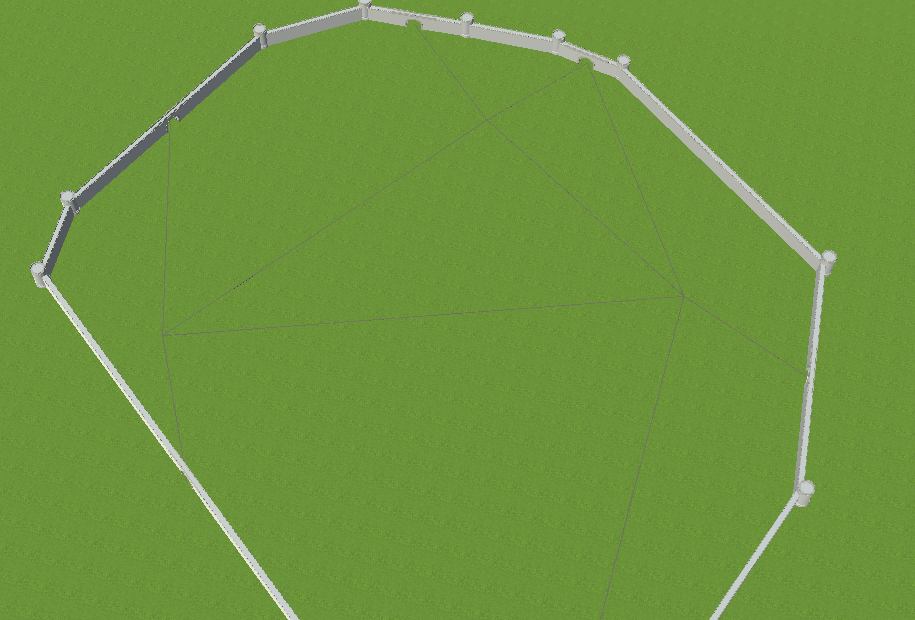
\includegraphics[width = 400px]{images/routeprimaire.png}
  \captionof{figure}{\small{Exemple d'une generation d'une route primaire}}
\end{center}


\subsection{L-systeme pour generation de route}
On va utiliser le système de lindenmayer (L-système) pour faire la génération de routes (principale et secondaire) qui est un système de réécriture qui comprend :

\begin{enumerate}
  \item Un alphabet V : l'ensemble des variables du L-système. On note V* l'ensemble des « mots » que l'on peut construire avec les symboles de V, et V+ l’ensemble des mots contenant au moins un symbole.
  \item Un ensemble de valeurs constantes S.
  \item Un axiome de départ w.
  \item Un ensemble de règles réécriture note P.
\end{enumerate}

Il est possible de construire une suite de mots à partir de l’axiome et des règles de dérivation en remplacant l'axiome par les règles un nombre 
definie de fois. \\

On s’inspire de l’interprétation en tortue \cite{flake2000computational} avec :

\begin{itemize}
  \item F : la tortue avance vers l’avant d’une distance fixe en dessinant un trait.
  \item G : la tortue avance vers l’avant d’une distance fixe sans dessiner de trait.
  \item + : la tortue tourne à droite d'un angle fixe.
  \item - : la tortue tourne à gauche d'un angle fixe.
  \item {[} : enregistrer la position courante de la tortue.
  \item {]} : revenir à la dernière position enregistrée et la supprimer de la pile de positions.
  \item | : la tortue avance vers l’avant d’une distance multipliée par une valeur en dessinant un trait.
\end{itemize}

On se base sur la même interprétation mais on modifie légèrement l’alphabet et on choisit des règles et un axiome propre a notre generation de terrain.
On choisit des valeurs de mouvement aléatoire pour ne pas avoir un même schéma qui se répète.

\textbf{Alphabet :}

\begin{itemize}
  \item F : Créer une route vers l’avant de l’axe Y d’une distance fixe.
  \item + : Créer une route vers la droite d’un angle fixe de 90.
  \item - : Créer une route vers la gauche d’un angle fixe de 90.
  \item {[} : enregistrer la position courante de la route.
  \item {]} : revenir à la dernière position enregistrée et la supprimer de la pile de positions.
  \item | : on avance vers l’avant d’une distance multipliée par une valeur en dessinant un trait.
\end{itemize}

On utilise l’axiome suivant : “+A-B” et pour avoir des routes différente à chaque exécution on utilise plusieur règles :

\begin{center}
  'A',"F[--AE]F[+AE]F" , 'A',"F[++EA]F[-AE]F" , 'A',"F[--EA]F[+AE]F",
\end{center} 

Sur chaque itération on choisit une règle aléatoirement qui nous permet d’avoir les résultats ci dessous.

\begin{center}
  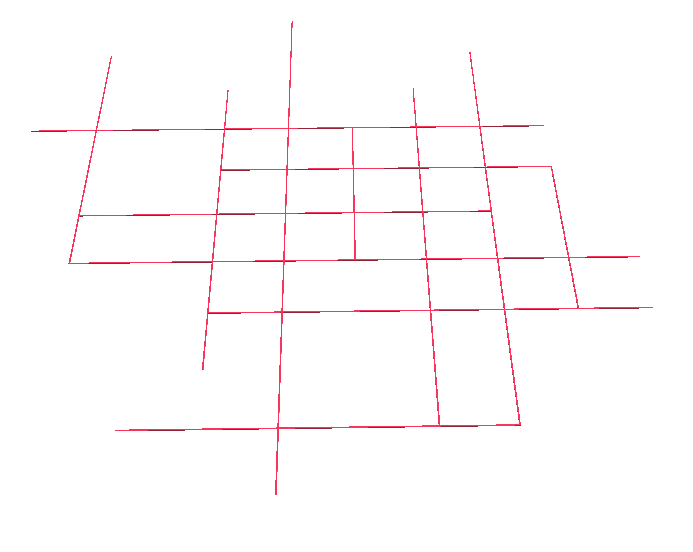
\includegraphics[width = 200px]{images/lsystem1.png}
  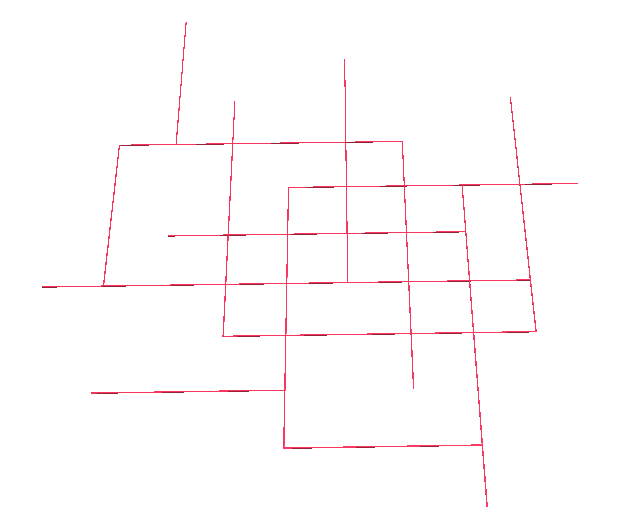
\includegraphics[width = 200px]{images/lsystem2.png}
  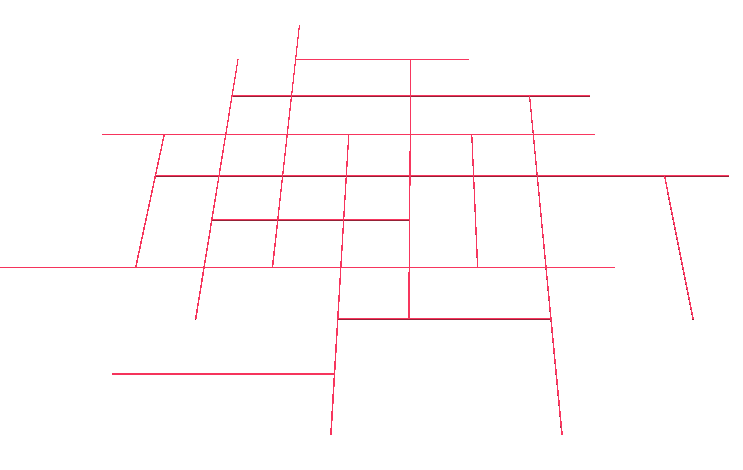
\includegraphics[width = 200px]{images/lsystem3.png}
  \captionof{figure}{\small{Exemple plusieur execution L-systeme}}
\end{center}

\newpage

\subsection{création de muraille qui entoure la ville}

L’algorithme nous permet principalement de définir l’endroit de la ville sur la map déjà générée qui se déroule comme ceci :\\

On commence par générer un point aléatoire vers le centre de la carte en divisant x et y par 2, on prend une valeur aléatoire qui servira de rayon aléatoire pour créer un cercle du point qu'on a pris comme centre. \\

On fait des pas aléatoire sur le périmètre du cercle qu'on vient de créer, c’est à dire qu’on se met aléatoirement sur une position du périmètre et on change l’angle, on aura des coordonnées $x$ et $y$ comme ceci $X =  rayon * cos(angle)$ | $Y = rayon * sin(angle)$.

Le fait de changer l’angle aléatoirement nous fait avoir des points $X$ $Y$ sur le long du périmètre du cercle, pour faire une plus grande variation entre les jonctions de la muraille, on crée depuis ses points des cercles avec un rayon plus petit que le rayon du premier grand cercle.

Pour chaque petit cercle créé sur le périmètre du premier grand cercle on génère un point aléatoire qui est défini par un angle et un rayon plus petit que le rayon du cercle.

\begin{center}
  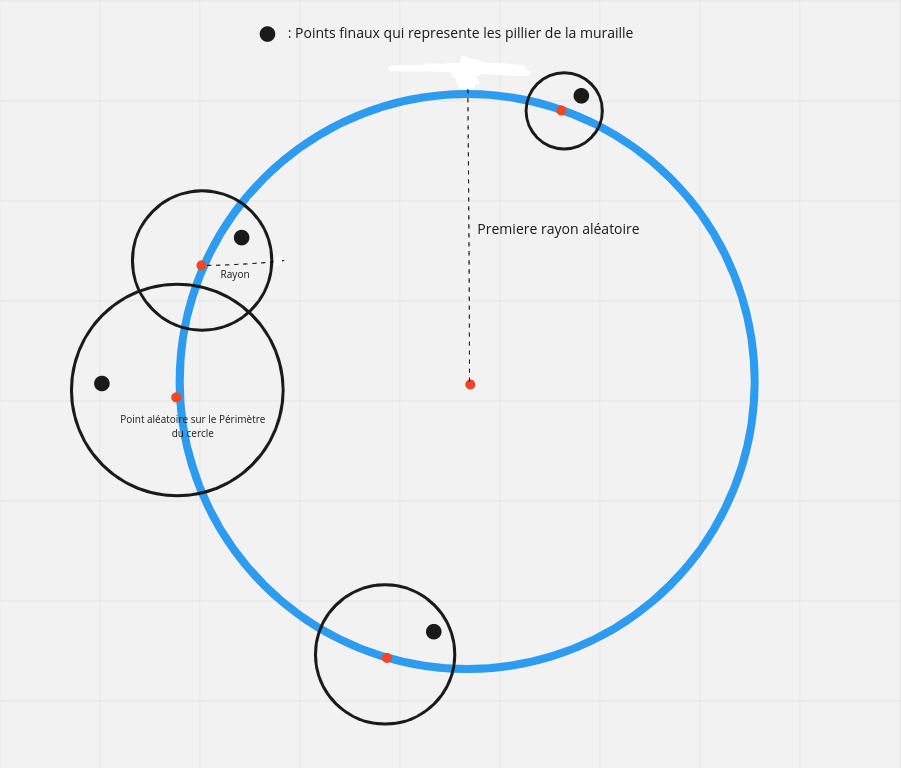
\includegraphics[height = 6 cm]{images/algorithme.png}
  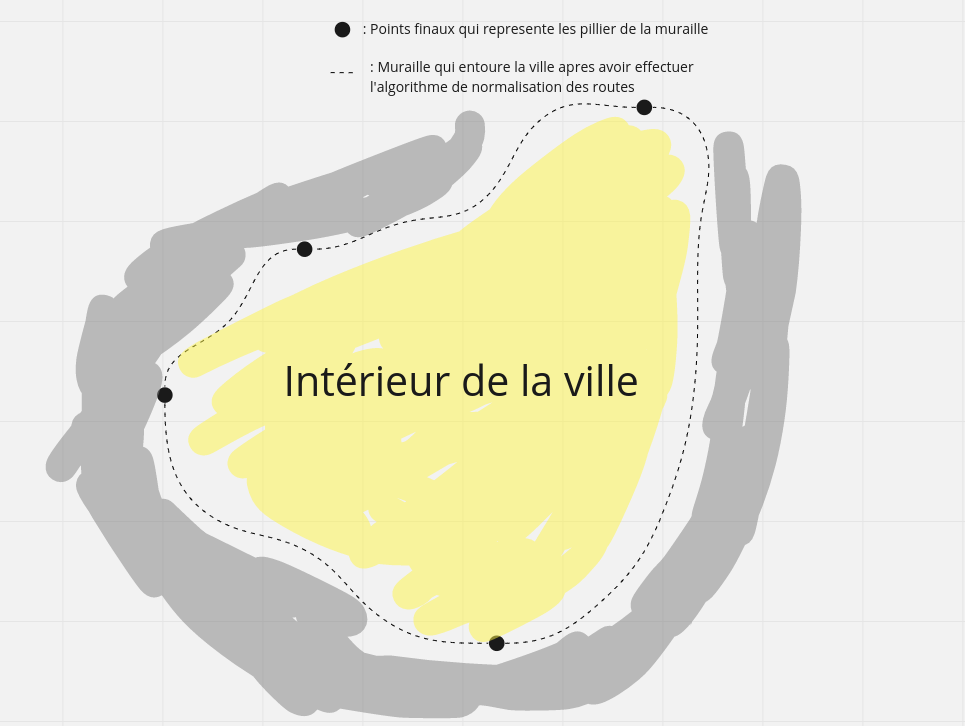
\includegraphics[height = 6 cm]{images/algo_final.png}\\
  \captionof{figure}{\small{ Déroulement de l'algorithme}}
\end{center}

\subsection{Algorithme d'échantillonnage}

Pour chaque point représentant le début A et la fin B d’une route, on prendra un rectangle d’une longueur à définir et d’une largeur de la taille entre A et B. On peut tracer le rectangle grâce au vecteur (A,B) qui nous permettra d’avoir le milieu.
On utilisera une de ses stratégies de sélection d'échantillonnage de routes pour sélectionner le chemin à prendre :\\

\begin{itemize}
  \item Stratégie d'élévation minimale : sélection de l'échantillon avec l'élévation (axe Z) la plus faible.
  \item Différence d'élévation la plus faible : On évite les chutes ou les montées d'altitude, et on cherche à maintenir une altitude régulière pour le segment de route complet. 
  \item Différence d'élévation moyenne : on sélectionne les points qui font une moyenne d’altitude.
\end{itemize}

Les trois stratégies sont contraintes d’avancer vers le point final en testant pour chaque nouveau point si on approche du point final.
Le choix se fait du prochain point se fait aléatoirement tant qu’il maintient une distance d’un seul point avec le points déjà selectionner.

Après la generation des points de murail on prends aléatoirement un nombre de porte qu’on crée au milieu des murs choisis aussi aléatoirement.

\begin{center}
  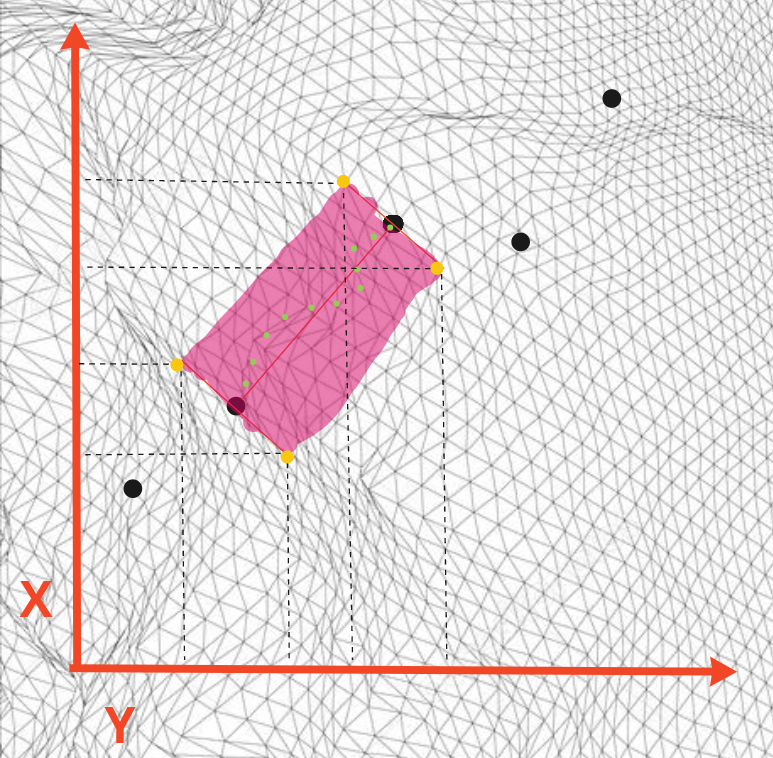
\includegraphics[height = 8 cm]{images/algo.png}\\
  \captionof{figure}{\small{ Déroulement de l'algorithme}}
\end{center}

\subsection{Algorithme de génération de bâtiments}

La génération de bâtiment se fait grâce à une bibliothèque de modèles médiévaux \cite{Assets}, elle contient plusieurs modèles qu’on va utiliser comme des bâtiments, arbres, etc.

La génération de bâtiments se fait en premier lieu autour des routes primaires et secondaires, grâce aux deux points qui représentent 
le début et la fin de la route, on peut obtenir la direction et la longueur qui nous permet de placer les bâtiments sur les deux côtés de la route, 
l’orientation se fait grâce au produit croisé du vecteur z avec la direction .
Les bâtiments sont placés d'un espace fixe de la route et d'un espace aléatoire des autres bâtiment précisé par l'utilisateur.

\begin{algorithm}
  \caption{Generer batiment}
  \KwData{Vecteur pointA, Vecteur pointB}
  
  float distance = pointB - pointA\;
  Vecteur orientation = cross((pointA - pointB) , (0,0,1))\;

  \For{int i = 0 ; i < distance ; i += tailleBatiment}
  {
    int position = Random(-espace,espace)\;
    i += position\;
    AfficherBatiment(pointA, position, orientation)\;
  }

  return;
\end{algorithm}

\newpage

\subsection{Algorithme de création de relief}

L’algorithme de l’interpollation linéaire (à ne pas confondre avec l’interpolation cubique qui lui lisse le relief) consiste à ajouter une courbe dans laquelle on a établi des points de pic ou de creux , pour établir une surface en relief, dans laquelle on y ajoutera des textures pour ressembler le plus à la description de l’objet que l’on veut établir , on va parler de bruits de turbulences, qui vont permettre d’ajouter le plus de détails possible à l’objet. Pour établir ce bruit on utilisera l’algorithme Perlin Noise : le but de cet algorithme et de créer une texture que l’on pourra utiliser comme effet visuel pour augmenter le réalisme de l’objet utilisé. L'algorithme peut être utilisé avec plusieurs dimensions et il consiste à calculer la produit scalaire de vecteurs gradiants que l'on aura mis en place sur une grille au préalable et de créer une interpolation de ces valeurs pour obtenir de nouvelles coordonnées et ainsi avoir un relief.

On va créer à partir d'un nuage de point de coordonnées (x,y) une fonction établissant la courbe entre chacun de ses points : 

La fonction $\bar{f}$ est définie par

\begin{center}
  ${\displaystyle {\bar {f}}(x)={\frac {y_{a}-y_{b}}{x_{a}-x_{b}}}x+{\frac {x_{a}\cdot y_{b}-x_{b}\cdot y_{a}}{x_{a}-x_{b}}}}$ \\
\end{center}

Une fois les calculs établis on obtient une courbe qui va alors nous permettre de créer un terrain en relief : 

\begin{center}
  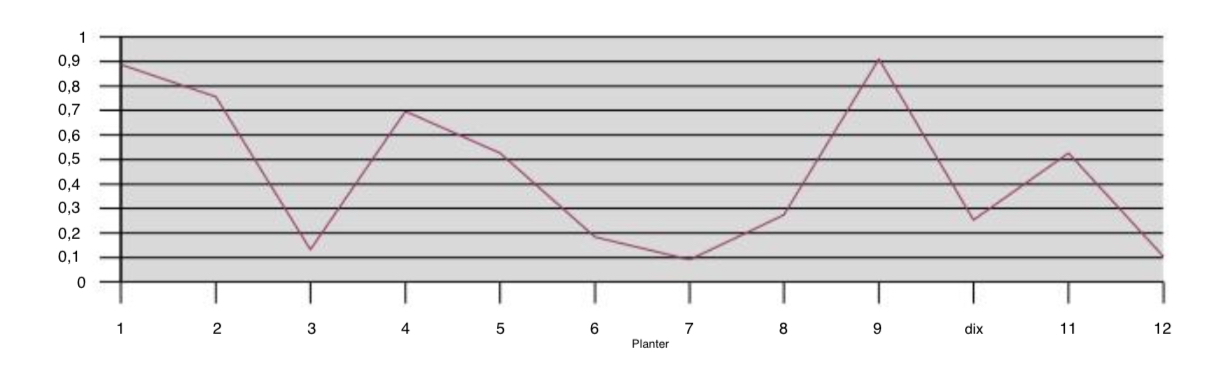
\includegraphics[height = 4 cm]{images/interlineaire.jpeg}\\
  \captionof{figure}{\small{Exemple de courbe par l'interpolation linéaire}}\cite{Kelly}
\end{center}

Le principe de l'interpolation s'établi à partir d'une formule qui peut être quelconque, le but est simplement d'obtenir de nouvelles valeurs de x et y, la formule ne doit pas être linéaire car on cherche à obtenir un terrain en relief et donc des coordonnées de hauteurs différentes pour chaque point, elle doit aussi donner des résultats similaires pour éviter d'avoir de trop grands écarts entre chaque point et ainsi obtenir un relief qui a des points trop elevés et d'autre trop faibles.

\subsection{Bruit de Perlin pour la création de relief}
On va utiliser le bruit de Perlin pour créer la génération du terrain.  

Le bruit de Perlin est une formule qui permet de créer une texture procédurale utilisée pour créer un effet visuel de réalisme. La fonction a une apparence de pseudo-aléatoire, mais c'est tout à fait le contraire, la texture produit un rendu "désordonné".

L'algorithme consiste à former une fonction de bruit qui, à une valeur donnée, associe une valeur qui semble aléatoire. Les valeurs obtenues sont donc liées aux valeurs de rentrée. 

Le résultat pourra être reproduit dans une deuxième texture si on insère les mêmes valeurs utilisées pour générer la texture précédente (à moins que le changement soit voulu ou effectué par un algorithme tierce).\\

C'est l'utilisation des paramètres tiers qui nous permettra d'obtenir un jeu de valeurs aléatoires pour qu'un observateur ne puisse pas trouver un motif qui se répète à certains intervalles. La difficulté réside dans le fait qu'on doit créer des valeurs aléatoires qui ont un rendu "désordonné". 

L'algorithme se décompose en deux étapes:
\begin{enumerate}
	\item Grille avec les gradients aléatoires : 
		l'algorithme forme une fonction f:N -> R qui, à une valeur donnée associe une valeur qui semble aléatoire. Cette caractéristique permet de reproduire le même résultat dans une deuxième texture si on insère les mêmes valeurs utilisées pour générer la texture précédente (à moins que le changement soit voulu ou effectué par un algorithme tierce).\\

\begin{center}
    \centering
    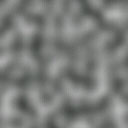
\includegraphics[height = 3 cm]{images/Perlin_noise.jpg}
    \captionof{figure}{Bruit de Perlin en deux dimensions \cite{berlinNoise}}
\end{center}

	\item Interpolation : 
	L'interpolation est « une opération mathématiques permettant de construire une courbe à partir des données d'un nombre fini de points ». Cette opération nous permet de créer une structure connectant chacune des coordonnées entre elles et produire un "maillage" qui sera utilisable lors de la création d'une surface.

\end{enumerate}

\begin{center}
    \centering
    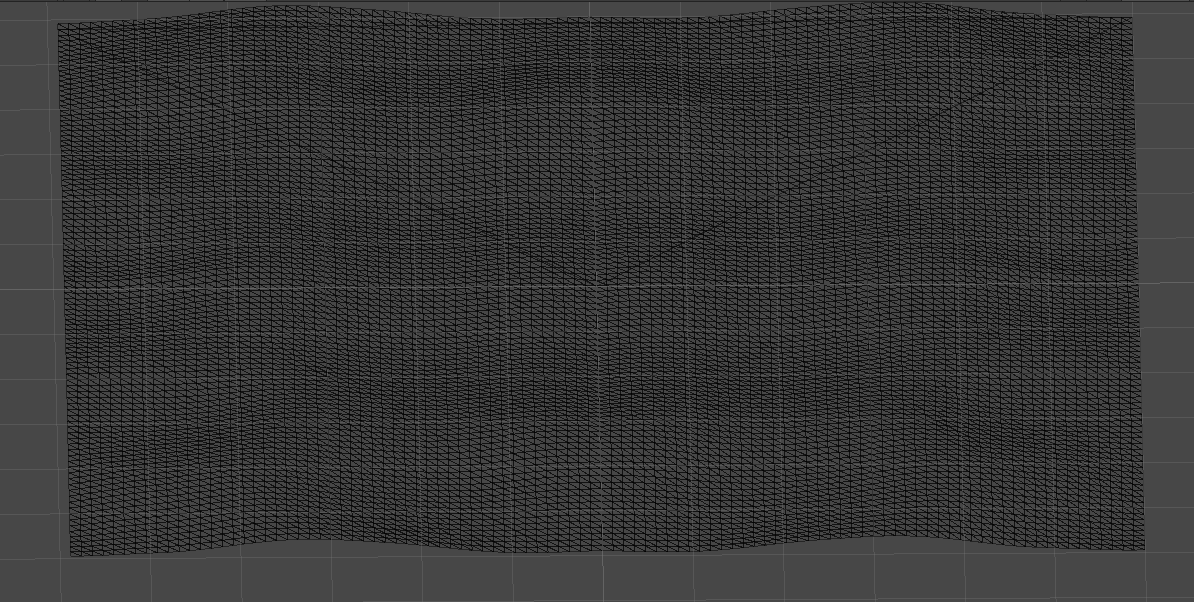
\includegraphics[height = 3 cm]{images/exemple_maillage.png}
\end{center}


Pour rendre le résultat avec plus de détails on peut implémenter les modifications suivantes: 

\begin{itemize}

\item Amplitude: Si on regarde la courbe point d'un point A à un B du terrain on observe que les valeurs (x, y, z) forment une courbe, le problème de ce dernier c'est que le terrain manque de perturbations.
	
     Pour cela on utilisera des octaves pour créer une irrégularité dans la texture. Les octaves c'est l'ensemble de courbes (créées par le bruit de Perlin) qui vont être utilisées pour former une courbe de forme quelconque. Pour cela on utilisera de la lacunarité et la persistance.
    
\item Lacunarité: Chaque octave pose une fréquence différente, donc les courbes produites sont différentes les unes des autres. La courbe utilisée pour créer une montagne doit avoir une fréquence plus grande que celle d'une colline car si la fréquence d'une montagne est petite avec une altitude élevée alors on obtient un pic dans le terrain.

\begin{center}
\centering
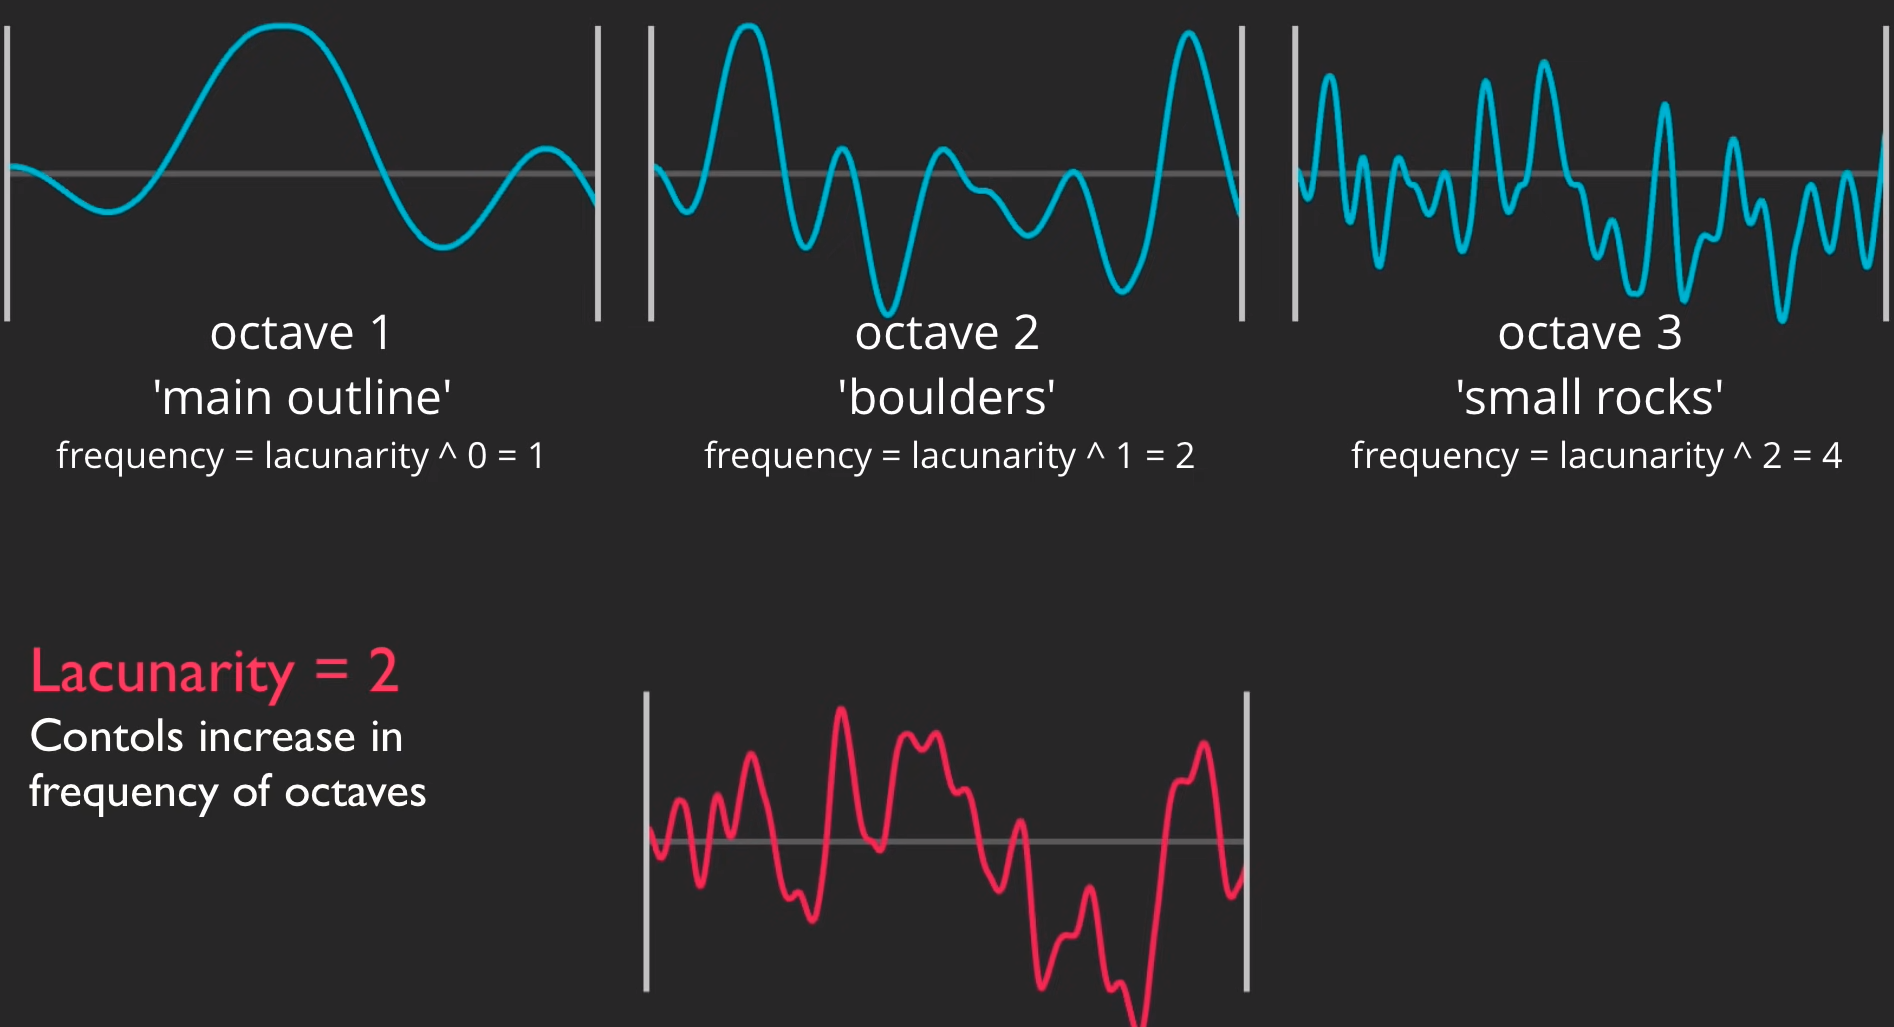
\includegraphics[height = 3 cm]{images/lacunarity.png}
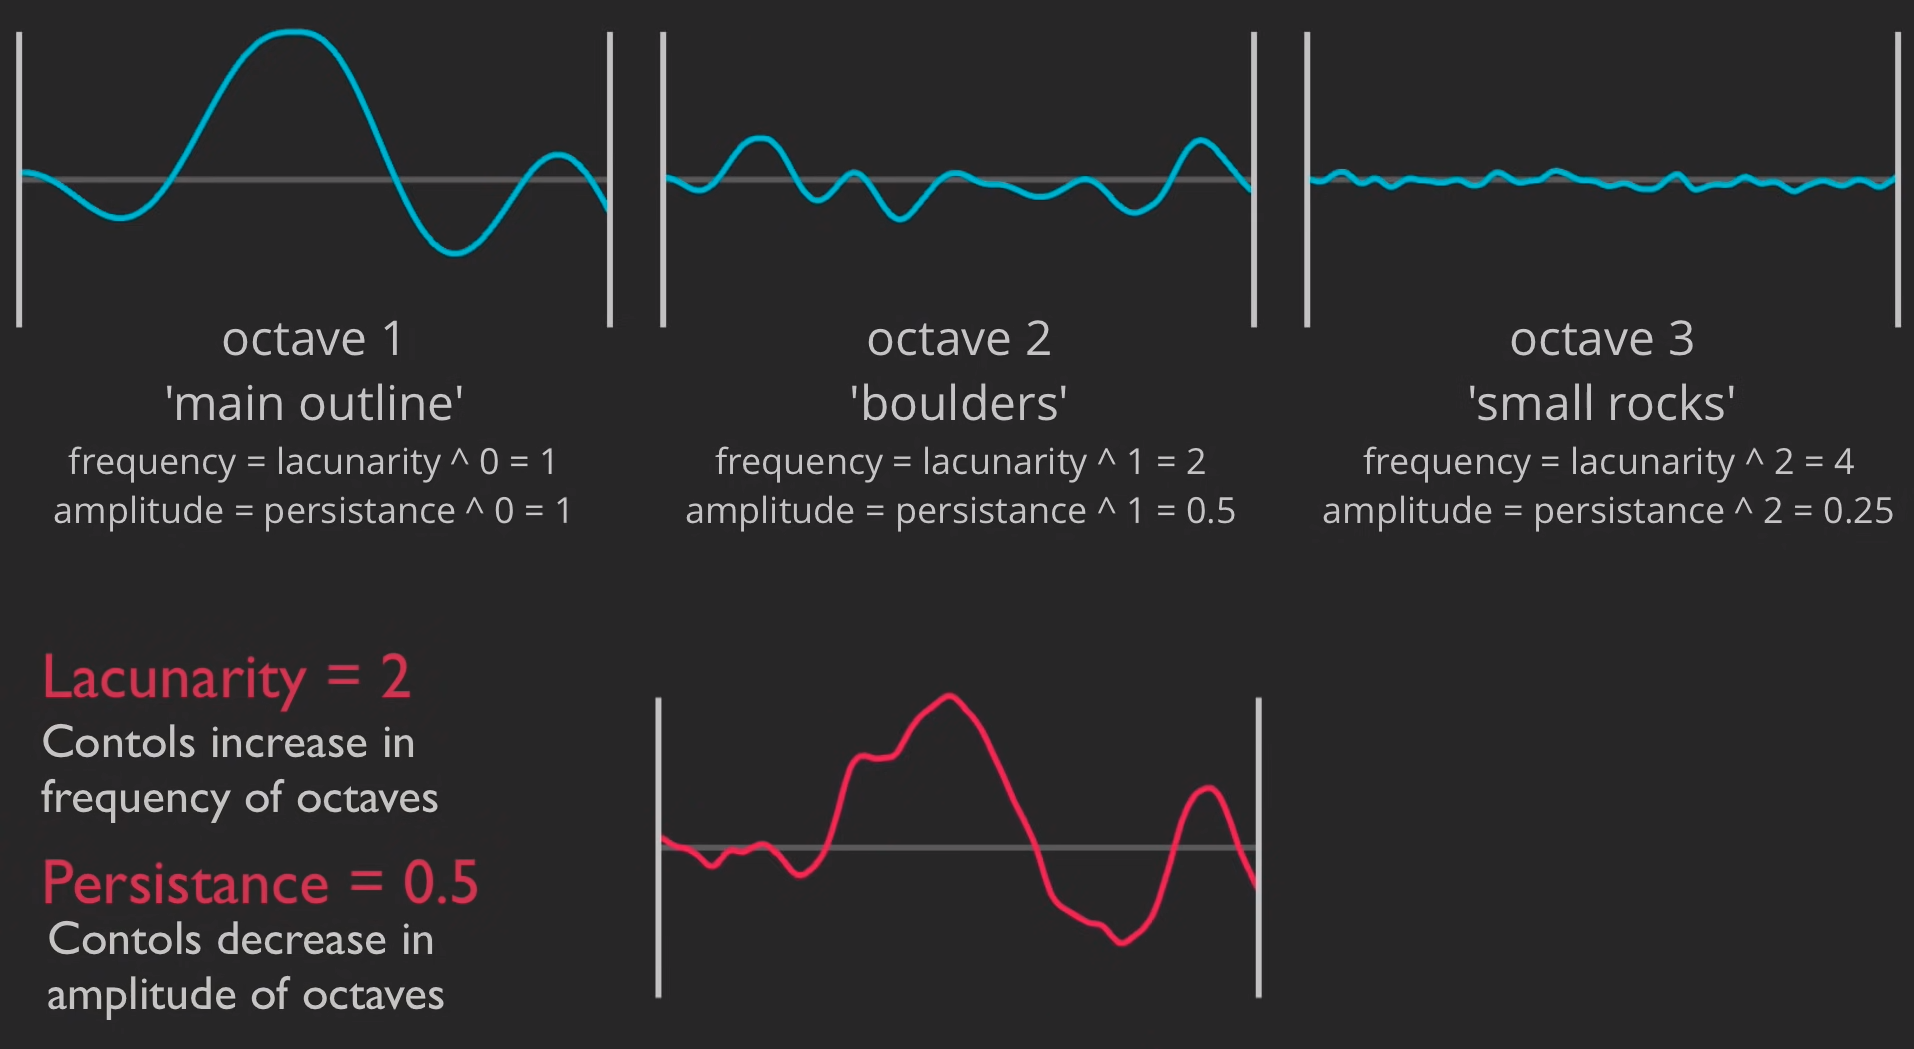
\includegraphics[height = 3 cm]{images/persistance.png}\\
\captionof{figure}{\small{Courbe bruit de Perlin avec amplitude.} \cite{lewisUnity}}
\captionof{figure}{\small{Courbe bruit de Perlin avec persistance.} \cite{lewisUnity}}
\end{center}

\item Persistance: c'est la fréquence (ou influence) des octaves sur la courbe principale. Chaque octave possède une importance sur le terrain, c'est-à-dire, l'octave qui sera utilisée pour 
créer des imperfections superficielles était moins importantes que l'octave utilisée pour ajouter des collines. 

\end{itemize}

\begin{center}
    \centering
    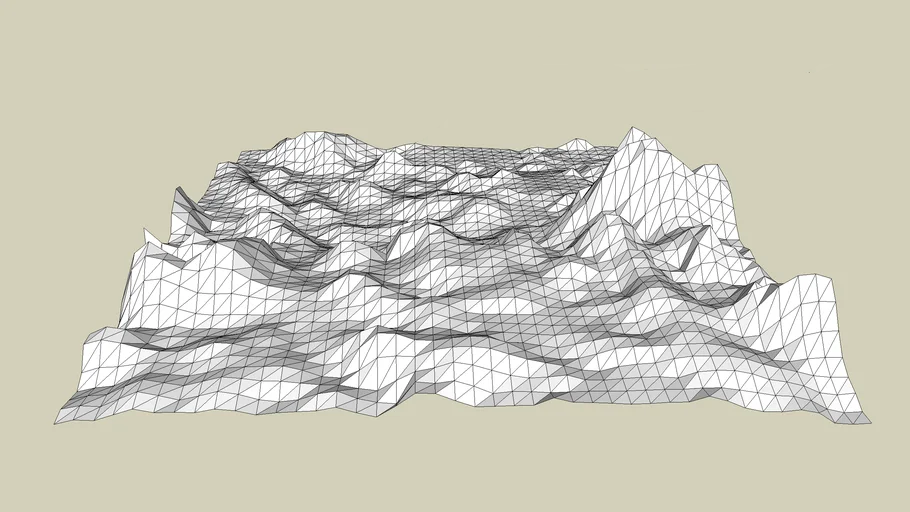
\includegraphics[height = 3 cm]{images/terrain3d.png}\\
    \captionof{figure}{\small{Exemple de représentation d'un terrain.} \cite{modelTerrain}}
\end{center}

Après avoir suivi les étapes précédentes on devrait avoir un terrain utilisable pour commencer à contruire les routes et le village.


La génération du terrain est un système qui comprend : 

\begin{itemize}
  \item Un tableau de taille (longueur x largeur) avec la valeur de la hauteur du point dans le terrain.
\end{itemize}

La tableau sera généré grâce à la fonction Mathf.Noise (fonction dans les bibliothèques de l'application Unity (moteur de jeu)) qui nous permet d'obtenir une suite de valeurs en utilisant la fonction du Bruit de Perlin.

\begin{center}
  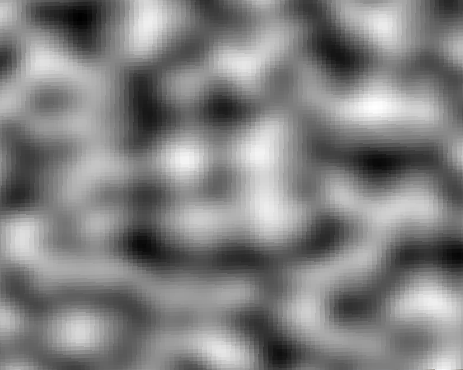
\includegraphics[width = 200px]{images/bruit_perlin_unity.png}
  \captionof{figure}{\small{Exemple d'une image produite sur unity en utilisant le bruit de Perlin}}
\end{center}

L'image est analysée de la manière suivante : la hauteur est codée avec une valeur allant de 0 à 1, plus on se rapproche de 0 plus on aura une couleur blanche et plus on se rapproche du 1 plus on aura une couleur noire.

\begin{algorithm}
  \caption{Bruit de Perlin}
  \KwData{coordonnées x, y}
  \KwResult{coordonnées x, y}
 
  initialisation \;
  
  grille[k] = (x,y); //vecteur gradiant
  
  \For{int i = 0; i < n; i++}{
  	distance[i] = |grille[i] - grille[k]| //vecteur distance \;
	int x1, y1 = produitScalaire(grille[k],distance[i]) \;
	interpolation(x1, y1)
  }
  	retourner x1\, y1\;
\end{algorithm}
% Algo MCB

\subsection{Algorithme MCB}
  
  L’algorithme MCB (Monte-Carlo Localization Boxed) nous permet de créer les City Cells en déterminant les boucles fermées du graphe des routes primaires.\\
  La création d'une liste d’adjacence de tout chaque points des routes principales nous permet d’avoir toutes les connexions des points.
  On commence par un point A et le un point B de sa liste d’adjacence, on prend la list d’adjacence du point B et on prend le point après 
  le point A, si le point A est a la fin de la list on prend le premier point de la list, jusqu'à retrouver le point A.

  Cet Algorithme nous retourne une liste de point qui forme les cellules de la ville, ce qui vas etre utile pour afficher les routes secondaire dedans.
   
  \begin{algorithm}
    \caption{Algorithme MCB}
    \KwData{List<Vecteur> listAdjacence , Vecteur pointA, Vecteur pointB}
    \KwResult{List<Vecteur> cellule}
    Vecteur pointDepart = pointA\;
    bool trouver = false\;

    \While{!trouver}
    {
      cellule.Ajouter(pointA);

      \ForEach{point dans listAdjacence[pointB]}
      {
        \If{!premiereExecution() and listAdjacence[pointB].contient(pointDepart)}
        {
          trouver = true;
        }
        \If{point == pointA}
        {
          Vecteur prochainPoint = point.Prochain();
          pointA = pointB;
          pointB = prochainPoint;
        }
      }
    }

    return listAdjacence\;

  \end{algorithm}
  
  
\begin{center}
  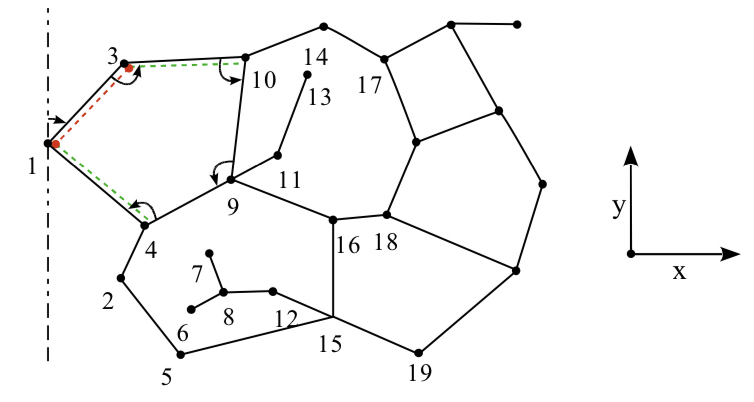
\includegraphics[height = 7 cm]{images/MCB.png}\\
  \captionof{figure}{\small{L'algorithme MCB \cite{Kelly}}}
  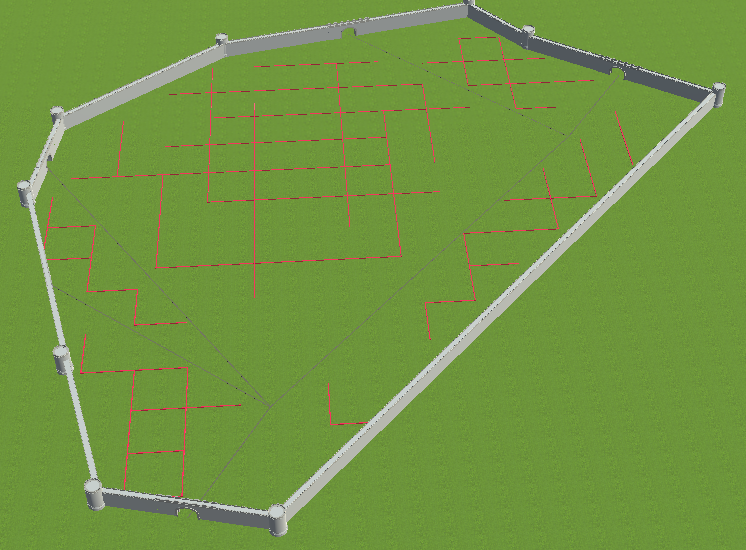
\includegraphics[height = 7 cm]{images/routeprimaireetsecondaire.png}\\
  \captionof{figure}{\small{Utilisation de cellules pour generer routes secondaire}}
\end{center}

